% arara: pdflatex
\documentclass[conference, 10pt]{IEEEtran}
\IEEEoverridecommandlockouts

% Memanggil file konfigurasi
\usepackage{preamble}

\begin{document}

\title{Analisis Penggunaan Gram Matrix dan CNN dalam Algoritma Neural Style Transfer untuk Sintesis Citra Artistik\\}

\author{\IEEEauthorblockN{Narendra Dharma Wistara M. \\ 
    NIM: 13524044\textsuperscript{1,2}}
\IEEEauthorblockA{
    Program Studi Teknik Informatika \\
    Sekolah Teknik Elektro dan Informatika \\
    Institut Teknologi Bandung, Jl. Ganesha 10 Bandung 40132, Indonesia \\
    \href{mailto:13524044@std.stei.itb.ac.id}{\color{blue}\textsuperscript{1}\textit{13524044@std.stei.itb.ac.id}}, 
    \href{mailto:andradaffamarpaung@gmail.com}{\color{blue}\textsuperscript{2}\textit{andradaffamarpaung@gmail.com}}}
}

\maketitle
\thispagestyle{fancy}

\begin{abstract}
   Makalah ini membahas peran Matriks Gram dan Convolutional Neural Network (CNN) dalam algoritma \textit{Neural Style Transfer} (NST) untuk sintesis citra artistik. Citra digital terlebih dahulu direpresentasikan sebagai tensor berdimensi tinggi sehingga setiap gambar dapat dipandang sebagai elemen ruang vektor, kemudian dipetakan oleh CNN (VGG-19) menjadi \textit{feature map} pada berbagai kedalaman layer yang membedakan informasi konten dan gaya. Konten direpresentasikan oleh matriks fitur $F_c^l$ dan $F_g^l$ pada layer tertentu, sedangkan gaya dimodelkan melalui Matriks Gram $G_s^l$ dan $G_g^l$ yang menangkap korelasi antar kanal fitur dan bersifat simetris serta \textit{positive semi-definite}.
\end{abstract}

\begin{IEEEkeywords}
    neural style transfer, citra, gaya, matriks gram, aljabar linier, CNN VGG-19
\end{IEEEkeywords}

\section{Pendahuluan}
Sebuah gambar dapat dipandang dari segi semantiknya (isi atau konten dari citra) dan segi gaya artistiknya.
Segi semantik mencerminkan apa yang ada dalam gambar (objek, struktur, komposisi), sementara segi gaya mencerminkan bagaimana gambar tersebut dipresentasikan (tekstur, pola, palet warna).

\begin{figure*}[b]
    \centering
    \includegraphics[width=0.8\textwidth]{assets/contohnst-1.png}
    \caption{\href{https://www.linkedin.com/pulse/artificial-intelligence-applications-neural-style-transfer-mohan}{Contoh Aplikasi NST pada Lukisan Mona Lisa}}
    \label{fig:contoh_nst_1}
\end{figure*}

Dari pembagian tersebut, muncul sebuah permasalahan dalam pemrosesan citra, yaitu "Dapatkah sebuah citra dipertahankan konten semantiknya, tetapi gambar tersebut disintesis gayanya?"
Inilah yang disebut dengan transfer tekstur atau transfer gaya (\textit{style transfer}).
Tujuan dari transfer gaya ini adalah untuk mensintesis gaya dari gambar sumber sambil membatasi sintesis gaya, sehingga konten semantik gambar target tetap terjaga. Dengan kata lain, kita ingin mengubah bagaimana gambar ditampilkan, tanpa mengubah apa yang ada dalam gambar tersebut. 

Salah satu perkembangan teknologi yang menjadi salah satu solusi dalam masalah ini adalah \textit{Neural Style Transfer} (NST). 
Algoritma NST menggunakan \textit{deep neural netrorks} untuk transformasi citra secara otomatis, memungkinkan sintesis gaya yang realistis dan artistik.
Salah satu kegunaan NST untuk pembuatan karya seni buatan dari foto atau karya seni lainnya. Misalnya, dengan mentransfer penampilan atau gaya sebuah lukisan ke foto yang disediakan pengguna. 


NST merupakan contoh dari penggayaan citra (image stylization), suatu masalah yang telah diteliti lebih dari dua dekade dalam bidang \href{https://en.wikipedia.org/wiki/Non-photorealistic_rendering}{\textit{non-photorealistic rendering}}. 
NST pertama dipublikasikan dalam makalah "A Neural Algorithm of Artistic Style" oleh Leon Gatys, dkk. pada tahun 2015. Algoritma ini memungkinkan komputer untuk memisahkan dan menggabungkan kembali konten visual dari satu citra dengan gaya artistik dari citra lain, menciptakan karya seni digital baru yang memukau. Contoh konkret dari aplikasi ini adalah mentransfer gaya lukisan "Mona Lisa" karya Leonardo da Vinci menjadi gambar yang tetap mempertahankan identitas subjek, tetapi dengan karakteristik artistik yang berbeda (\ref{fig:contoh_nst_1}).


Meskipun sering dipandang sebagai aplikasi dari \textit{Deep Learning} dan \textit{Convolutional Neural Network} (CNN), fondasi utama yang memungkinkan NST bekerja adalah prinsip-prinsip matematika yang dipelajari dalam Aljabar Linier dan Geometri. Citra digital pada dasarnya adalah representasi matriks atau tensor berdimensi tinggi dalam ruang Euclidean. Proses ekstraksi fitur, manipulasi gaya, dan rekonstruksi citra dalam NST sangat bergantung pada operasi matriks, transformasi ruang vektor, dan perhitungan jarak antar vektor.

Dalam upaya mengatasi permasalahan pemisahan konten dan gaya, Gatys dkk. (2015) menemukan bahwa Matriks Gram adalah metode yang paling sesuai untuk merepresentasikan gaya secara matematis. Matriks Gram didefinisikan sebagai hasil perkalian inner product antara \textit{feature maps} dalam \textit{neural network}. Matriks Gram menyediakan cara yang sangat baik untuk menangkap karakteristik gaya sebagai korelasi statistik antar fitur, tanpa harus menyimpan informasi spasial. 

Makalah ini bertujuan untuk menganalisis peran Matriks Gram dalam algoritma \textit{Neural Style Transfer} dari sudut pandang Aljabar Linier. 
Penulis akan menganalisis bagaimana konsep-konsep Aljabar Linier seperti transposisi matriks, perkalian matriks, dan nilai eigen digunakan untuk memanipulasi informasi visual. 

\section{Dasar Teori}
\subsection{Tensor}
Dalam matematika, tensor didefinisikan sebagai objek geometris yang memetakan himpunan vektor dan kovektor ke dalam sebuah skalar secara linier. Dalam konteks \textit{Deep Learning} dan pengolahan data, tensor lebih sering dipahami sebagai generalisasi dari matriks ke dimensi yang lebih tinggi. Tensor adalah struktur data array multidimensi yang berfungsi sebagai wadah penampung data numerik. Karakteristik utama sebuah tensor ditentukan oleh \textit{Rank} (atau Orde) dan Bentuk/Dimensi-nya.
Secara hierarkis, struktur data dapat diklasifikasikan sebagai tensor dengan rank tertentu:
\begin{IEEEitemize}
    \item Tensor Rank-0 (Skalar) merupakan nilai tunggal (bilangan real). 
        Skalar hanya memiliki besaran (magnitudo) tanpa arah. Notasi matematikanya dapat dituliskan sebagai $x \in \mathbb{R}$.
    \item Tensor Rank-1 (Vektor) merupakan susunan bilangan dalam satu dimensi (\textit{Array 1D}). Vektor memiliki besaran dan arah dalam ruang. 
        Vektor di ruang Euclidean $\mathbb{R}^n$ dinyatakan sebagai $n$-tupel bilangan riil. Dalam matematika, ini dapat dinotasikan sebagai: $\mathbf{v} \in \mathbb{R}^n$
    \item Tensor Rank-2 (Matriks) merupakan susunan bilangan dalam dua dimensi (\textit{Array 2D}) yang terdiri dari baris dan kolom. Matriks merepresentasikan transformasi linier antar ruang vektor. 
        Matriks berukuran $m \times n$ adalah tensor rank-2 dengan bentuk $(m, n)$. Tensor rank-2 dapat dinotasikan sebagai berikut: $A \in \mathbb{R}^{m\times n}$

    \item Tensor Rank-3 dan seterusnya, merupakan susunan bilangan dalam tiga dimensi atau lebih. 
        Tensor rank-3 sering dibayangkan sebagai kubus angka atau tumpukan beberapa matriks. 
\end{IEEEitemize}

Tensor biasanya dinotasikan dengan huruf kapital kaligrafi, misalnya $\mathcal{X}, \mathcal{Y}, \mathcal{Z}$.
Elemen individu dari sebuah tensor dapat diakses menggunakan indeks yang sesuai dengan jumlah dimensinya.
Misalkan $\mathcal{T}$ adalah sebuah tensor rank-3, maka elemen pada posisi $(i, j, k)$ dapat dinotasikan sebagai
$\mathcal{T}_{(i, j, k)}$

Visualisasi dari Tensor Rank-0 sampai Rank-3 dapat dilihat pada Gambar \ref{fig:contoh-tensor} berikut.
\begin{figure}[h]
    \centering
    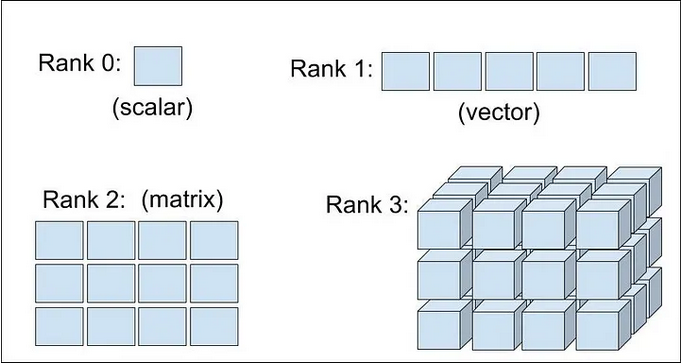
\includegraphics[width=0.4\textwidth]{assets/hierarki-tensor.png}
    \caption{\href{https://thefaheemkhan.medium.com/what-is-tensors-in-machine-learning-4cbf90490a7b}{Visualisasi Tensor Rank-0 sampai Rank-3}}
    \label{fig:contoh-tensor}
\end{figure}

\subsection{Representasi Citra Digital}
Citra digital merupakan representasi diskrit dari suatu gambar kontinu yang telah disampel dalam bentuk grid dua dimensi yang tersusun atas elemen-elemen terkecil yang disebut pixel. Setiap pixel menyimpan informasi intensitas yang umumnya dinyatakan sebagai bilangan bulat, biasanya dapat berupa $[0, 255]$ atau $[0, 1]$ tergantung format penyimpanan dan pemrosesan.
Pada citra \textit{grayscale}, setiap pixel hanya memiliki satu intensitas yang menggambarkan tingkat kecerahan pada posisi tertentu.
Pada citra berwarna, khususnya pada format RGB (\textit{Red, Green, Blue} direpresentasikan oleh tiga komponen intensitas, masing-masing untuk kanal merah, hijau, dan biru. Ketiga nilai ini kemudian dikombinasikan untuk menghasilkan warna akhir pada pixel tersebut.

Secara umum pixel pada citra berwarna dapat dituliskan sebagai
$$
\begin {pmatrix}
    I_{R}(h, w) \\
    I_{G}(h,w) \\ 
    I_{B}(h,w)
\end{pmatrix}
$$

di mana \(I_R(h,w)\), \(I_G(h,w)\), dan \(I_B(h,w)\) menyatakan intensitas kanal merah, hijau, dan biru pada koordinat spasial \((h,w)\).

Pada citra skala keabuan (grayscale), informasi warna diabaikan, dan hanya intensitas cahaya yang disimpan. Citra ini direpresentasikan sebagai matriks.
$$
I \in \mathbb{R}^{H \times W}
$$

Setiap elemen matriks $I_{ij}$ menyimpan nilai skalar yang merepresentasikan kecerahan.

$$
I = \begin{bmatrix}
p_{11} & p_{12} & \cdots & p_{1W} \\
p_{21} & p_{22} & \cdots & p_{2W} \\ 
\vdots & \vdots & \ddots & \vdots \\
p_{H1} & p_{H2} & \cdots & p_{HW}
\end{bmatrix}
$$

Umumnya, nilai $p_{ij}$ dikuantisasi menjadi bilangan bulat dalam rentang $[0,255]$ untuk citra 8-bit, di mana nilai 0 merepresentasikan hitam sempurna dan 255 merepresentasikan putih sempurna.

Pada citra berwarna, umumnya tiap piksel dalam gambar tersusun atas tiga komponen warna dasar, yaitu merah (\textit{red}), hijau (\textit{green}), dan biru (\textit{blue}) atau yang biasa disingkat RGB. 
Sama seperti pada representasi citra \textit{greyscale}, setiap komponen tersebut dapat direpresentasikan dalam rentang nilai 0 hingga 255.
Namun, citra berwarna tidak cukup direpresentasikan oleh satu matriks. Citra berwarna berukuran $H \times W$ direpresentasikan sebagai Tensor Orde-3.
$$
I \in \mathbb{R}^{H \times W \times 3}
$$ 

Setiap piksel pada posisi $(i, j)$ bukan lagi sebuah skalar, melainkan sebuah vektor $\textbf{v} \in \mathbb{R}^{3}$.

$$
\mathbf{v}_{H, W} = 
\begin{pmatrix}
r_{(HW)} \\
g_{(HW)} \\
b_{(HW)} 
\end{pmatrix}
$$

Di mana  $r, g, b$ adalah intensitas masing-masing kanal warna. Dengan demikian nilai $I(h, w, c)$ menyatakan intensitas kanal ke-$c$ pada posisi $(h, w)$ dengan $c$ menyatakan kanal warna (misalnya, R, G, dan B).

Lebih umum, citra dengan \(C\) kanal (misalnya RGB, RGBA, atau representasi fitur lain) dapat ditulis sebagai tensor rank‑3.
$$
I \in \mathbb{R}^{H \times W \times C}.
$$

\subsection{Matriks Gram}

Misalkan diberikan $n$ buah vektor $\mathbf{v}_1, \mathbf{v}_2, \ldots, \mathbf{v}_n \in \mathbb{R}^m$.
Matriks Gram $G \in \mathbb{R}^{n \times n}$ didefinisikan sebagai matriks yang elemen-elemennya adalah hasil kali dalam (inner product) antara setiap pasangan vektor:
$$
    G_{ij} = \langle \mathbf{v}_i, \mathbf{v}_j \rangle, \qquad 1 \leq i,j \leq n.
$$

Jika vektor-vektor tersebut disusun sebagai kolom-kolom dari sebuah matriks
$$
    V =
    \begin{pmatrix}
        \vert & \vert &        & \vert \\
        \mathbf{v}_1 & \mathbf{v}_2 & \cdots & \mathbf{v}_n \\
        \vert & \vert &        & \vert
    \end{pmatrix}
    \in \mathbb{R}^{m \times n},
$$
maka matriks Gram dapat ditulis ringkas sebagai
$$
    G = V^\top V.
$$
Dengan demikian, matriks Gram dapat dipandang sebagai matriks yang merangkum seluruh inner product antara vektor-vektor pada kolom matriks $V$.

Secara geometris, elemen-elemen matriks Gram memiliki makna sebagai berikut. Untuk setiap elemen diagonal $G_{ii}$ menyatakan kuadrat norma (panjang) vektor $\mathbf{v}_i$. 
$$
    G_{ii} = \langle \mathbf{v}_i, \mathbf{v}_i \rangle = \Vert \mathbf{v}_i \Vert_2^2
$$

Sedangkan, untuk elemen nondiagonal $G{ij}$ menyatakan sudut antara $\mathbf{v}_i$ dan $\mathbf{v}_j$.
$$
    G_{ij} = \langle \mathbf{v}_i, \mathbf{v}_j \rangle = \Vert \mathbf{v}_i \Vert_2  \cdot \Vert \mathbf{v}_j \Vert_2 \cdot \cos(\theta_{ij})
$$

Nilai $G_{ij}$ mengukur tingkat keselarasan (korelasi) antara dua vektor. Semakin besar nilai $G_{ij}$, maka semakin searah kedua vektor (menunjukkan korelasi yang kuat. Sebaliknya, semakin kecil nilai $G_{ij}$, maka semakin tidak searah kedua vektor (menunjukkan korelasi yang rendah). Jika, $G_{ij} \approx 0$, maka kedua vektor hampir orthogonal (sudut hampir mendekati $90^\circ$. Dengan demikian, matriks Gram dapat dipandang sebagai matriks korelasi (berbasis inner product) yang menangkap hubungan geometris antar vektor di dalam suatu himpunan.

Matriks Gram memiliki beberapa sifat sebagai berikut.
\begin{enumerate}
    \item Matriks Gram merupakan matriks simetris. Dari definisi,
    \[
        G_{ij} = \langle \mathbf{v}_i, \mathbf{v}_j \rangle
        = \langle \mathbf{v}_j, \mathbf{v}_i \rangle = G_{ji},
    \]
    sehingga diperoleh $G = G^\top$.

\item Matriks Gram bersifat \href{https://en.wikipedia.org/wiki/Definite_matrix}{Positive semi-definite}.
    Untuk setiap vektor $\mathbf{x} \in \mathbb{R}^n$ berlaku
    $$
        \mathbf{x}^\top G \mathbf{x}
        = \mathbf{x}^\top V^\top V \mathbf{x}
        = \| V \mathbf{x} \|_2^2 \geq 0.
    $$
    Konsekuensinya, semua nilai eigen dari $G$ tidak negatif. $\lambda_k \ge 0$ untuk setiap nilai eigen $\lambda_k$ dari $G$

    \item Matriks Gram dapat didiagonalisasi secara orthogonal. Akibat $G$ simetris dan positive semi-definite, $G$ dapat didekomposisi secara orthogonal:
    $$
        G = Q \Lambda Q^\top,
    $$
    dengan $Q$ matriks orthogonal yang kolom-kolomnya adalah vektor-vektor eigen yang ternormalisasi, dan $\Lambda$ matriks diagonal yang berisi nilai-nilai eigen $\lambda_1, \ldots, \lambda_n$. Nilai eigen besar dapat ditafsirkan sebagai komponen utama yang dominan dalam struktur korelasi yang direpresentasikan oleh $G$.
\end{enumerate}

\subsection{Fungsi Loss}

Fungsi \textit{Loss} (\textit{Loss Function}) adalah fungsi yang mengukur seberapa jauh keluaran suatu model atau suatu variavel keputusan dari nilai yang diinginkan. Secara umum, fungsi \textit{loss} memetakan pasangan prediksi dan target ke sebuah bilangan riil tak negatif.
$$
L_{\text{prediksi}, \text{target}} \in \mathbb{R}_{\ge 0}
$$

Semakin kecil nilai \textit{loss}, semakin baik kesesuaian antara prediksi dan target.

Salah satu bentuk \textit{loss} yang paling dasar adalah loss berbasis jarak Euclidean. Misalkan $y, \hat{y} \in \mathbb{R}^{n}$ masing-masing menyatakan vektor target dan vektor prediksi. Jarak Euclidean antara keduanya didefinisikan sebagai:
$$
    d(y, \hat{y}) = \Vert y - \hat{y} \Vert_2 = 
    \sqrt{ \sum_{i=1}^{n} (y_i - \hat{y}_i)^2 }.
$$

Dalam banyak algoritma optimasi, sering digunakan \textit{squared Euclidean distance}, karena bentuk kuadrat ini lebih sederhana untuk dianalisis dan diturunkan gradiennya.
$$
    d(y, \hat{y})^2 = \Vert y - \hat{y} \Vert_2^2 = \sum_{i = 1}^n (y_1 - \hat{y}_i)^2
$$

Bentuk umum loss semacam ini dikenal sebagai \textit{mean squared error} (MSE) ketika nilai kuadrat perbedaan rata-ratanya yang digunakan:
\[
    L_{\mathrm{MSE}}(y, \hat{y}) 
    = \frac{1}{n} \sum_{i=1}^{n} (y_i - \hat{y}_i)^2.
\]

Konsep yang sama dapat diperluas ke matriks. Misalkan $A, B \in \mathbb{R}^{m \times n}$. Salah satu ukuran perbedaan yang sering digunakan adalah norma Frobenius:
$$
    \| A - B \|_F^2 
    = \sum_{i=1}^{m} \sum_{j=1}^{n} (A_{ij} - B_{ij})^2.
$$

Jika diperlukan, loss antara dua matriks dapat didefinisikan langsung sebagai
$$
    L(A,B) = \| A - B \|_F^2.
$$

\subsection{Convolutional Neural Network (CNN)}
\textit{Deep Learning} berarti jaringan saraf (\textit{neural network} yang memiliki banyak lapisan tersembunyi (\textit{hidden layers}. Kedalaman atau jumlah lapisan ini memungkinkan sebuah jaringan mempelajari representasi fitur yang semakin abstrak Secara matematis, jika sebuah neuron menerima vektor masukan 
$$
\mathbf{x} = (x_1, x_2, \ldots, x_n)^\top
$$
dengan bobot
$$
\mathbf{w} = (w_1, w_2, \ldots, w_n)^\top
$$
dan bias $b$, maka keluarannya $z$ dapat ditulis sebagai
$$
z = \sigma(\mathbf{w}^\top \mathbf{x} + b),
$$

Proses pembelajaran dilakukan dengan meminimalkan fungsi \textit{loss} menggunakan algoritma optimasi dengan cara menyesuaikan bobot dan bias agar keluaran jaringan mendekati target yang diinginkan. 

Convolutional Neural Network (CNN) adalah jenis \textit{deep neural network} yang dirancang khusus untuk memproses data yang memiliki struktur spasial, seperti citra dua dimensi. Berbeda dengan jaringan saraf berlapis penuh (fully-connected network) yang menghubungkan setiap neuron pada satu lapisan ke semua neuron di lapisan berikutnya, CNN menggunakan operasi konvolusi dengan filter (kernel) berukuran kecil yang digeser (sliding) di atas citra atau \textit{feature maps}.

Pada sebuah \textit{convolutional layer}, diberikan tensor masukan berdimensi
$$
H \times W \times C_\text{in},
$$
serta sekumpulan filter berukuran kecil (misalnya $3 \times 3$) dengan $C_\text{out}$ buah filter. Setiap filter menghasilkan satu \textit{feature map}, sehingga keluaran layer ini berupa tensor
$$
H' \times W' \times C_\text{out},
$$
di mana $H'$ dan $W'$ adalah tinggi dan lebar baru setelah operasi konvolusi (dan mungkin subsampling). Intuisi utama CNN adalah bahwa setiap filter belajar mendeteksi pola tertentu (misalnya tepi, tekstur, atau bentuk) pada berbagai lokasi spasial.

\begin{figure}[H]
    \centering
    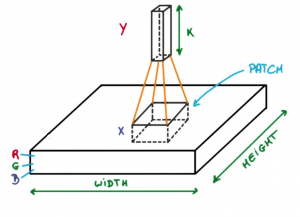
\includegraphics[width=0.4\textwidth]{assets/contoh-cnn.png}
    \caption{\href{https://www.geeksforgeeks.org/machine-learning/introduction-convolution-neural-network/}{Visualisasi \textit{Convolutional Layer}}}
    \label{fig:contoh-cnn}
\end{figure}


Sebuah Convolutional Neural Network (CNN) tersusun atas urutan beberapa lapisan, di mana setiap lapisan mengubah sebuah volume data tensor menjadi volume lain melalui fungsi yang terdiferensialkan. Untuk citra, volume ini biasanya memiliki dimensi tinggi, lebar, dan kanal (\textit{channel}) atau $H \times W \times C$.

\begin{IEEEitemize}
    \item \textit{Input layer}. Layer ini menampung data mentah yang diberikan ke jaringan. Pada lapisan ini belum ada komputasi selain penyediaan data untuk lapisan berikutnya.
    \item \textit{Convolutional layer}. Layer ini bertugas mengekstraksi fitur dari citra. Lapisan ini memiliki sekumpulan filter (kernel) berukuran kecil, misalnya $3 \times 3$ yang digeser di atas citra. Untuk setiap posisi, filter dan \textit{patch} citra yang bersesuaian dikalikan elemen per elemen, lalu dijumlahkan, menghasilkan satu nilai pada pada \textit{feature map}
    \item \textit{Activation layer}. Layer ini menerapkan fungsi aktivasi nonlinier pada tiap elemen pada keluaran \textit{convolutional layer}. Fungsi aktivasi yang umum digunakan, yaitu ReLU.
        $$
        \text{ReLU}(x) = \max(0, x)
        $$
    Lapisan ini tidak mengubah dimensi volume, tetapi penting agar jaringan memodelkan hubungan nonlinier yanag kompleks antar piksel.

    \item \textit{Pooling Layer}. Layer ini disisipkan secara berkala untuk mengecilkan ukuran dari \textit{feature maps}. Konsep utamanya adalah untuk merangkum informasi lokal di suatu submatrix kecil menjadi satu nilai. Dua jenis \textit{pooling} yang paling sering digunakan adalah \textit{max pooling} yang mengambil nilai maksimum dalam submatrix dan \textit{average pooling} yang mengambil nilai rata-rata dalam submatrix. 

    \item \textit{Flattening} dan \textit{fully connected layer}. Setelah beberapa kali konvolusi-aktivasi-pooling, biasanya volume fitur yang tersisa diubah menjadi vektor satu dimensi agar dapat dihubungkan ke lapisan \textit{fully connected}. Jika volume terakhir memiliki ukuran $H_f \times W_f \times C_f$, maka hasil flatten adalah vektor di $\mathbb{R}^{H_f \cdot W_f \cdot C_f}$. Lapisan ini kemudian memperlakukan vektor ini seperti masukan jaringan saraf biasa. Setiap neuron terhubung ke semua komponen vektor, dengan bobot dan bias masing-masing. Lapisan ini digunakan untuk klasifikasi, regresi, atau tujuan akhir lainnya. 

    \item \textit{Output layer}. Layer terakhir ini menerima keluaran dan mengubahnya menjadi bentuk yang sesuai dengan tugas.

\end{IEEEitemize}

\begin{figure}[H]
    \centering
    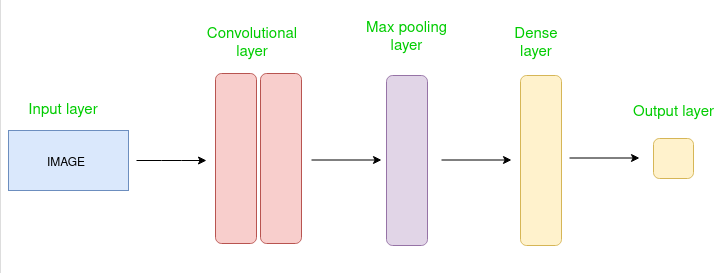
\includegraphics[width=0.4\textwidth]{assets/cnn-architecture.png}
    \caption{\href{https://www.geeksforgeeks.org/machine-learning/introduction-convolution-neural-network/}{Arsitektur CNN}}
    \label{fig:arsitektur-cnn}
\end{figure}

Dalam algoritma NST, arsitektur CNN yang digunakan adalah VGG-19. Baca: \url{https://www.sciencedirect.com/topics/computer-science/vgg-19-convolutional-neural-network} sebagai referensi

\subsection{Neural Style Transfer}
Neural Style Transfer (NST) adalah sebuah metode yang bertujuan untuk menghasilkan citra baru $I_g$ yang menggabungkan konten dari sebuah citra konten $I_c$ dan gaya dari sebuah citra gaya $I_s$. Secara intuitif, konten mengacu pada struktur global atau tata letak objek dalam gambar (bentuk, posisi, dan susunan besar), sedangkan gaya berkaitan dengan karakteristik visual seperti tekstur, pola sapuan kuas, dan skema warna.

Pendekatan NST memanfaatkan jaringan saraf konvolusional (CNN) yang telah dilatih sebelumnya (misalnya VGG-19) untuk memperoleh representasi fitur dari citra. Representasi ini kemudian digunakan untuk mendefinisikan \textit{content loss} dan \textit{style loss}, sehingga citra hasil $I_g$ dapat dioptimasi agar secara bersamaan mendekati konten $I_c$ dan gaya $I_s$.

% \subsection{Representasi Konten dengan VGG-19}
%
% Seperti telah dibahas pada bagian CNN dan arsitektur VGG-19, setiap layer konvolusi pada VGG-19 menghasilkan \textit{feature maps} yang dapat dianggap sebagai representasi fitur dari citra pada tingkat abstraksi tertentu. Misalkan untuk sebuah layer ke-$l$ diperoleh tensor fitur berdimensi
% $$
% C_l \times H_l \times W_l,
% $$
% yang selanjutnya di-reshape menjadi sebuah matriks
% $$
% F^l \in \mathbb{R}^{C_l \times (H_l W_l)},
% $$
% di mana setiap baris dari $F^l$ merepresentasikan satu kanal fitur, dan setiap kolom merepresentasikan satu posisi spasial.
%
% Untuk merepresentasikan konten, dipilih satu layer menengah (misalnya \texttt{conv4\textsubscript{2}}) yang dianggap menangkap struktur global citra dengan baik. Jika $F^l_c$ menyatakan matriks fitur pada layer ke-$l$ untuk citra konten $I_c$, dan $F^l_g$ menyatakan matriks fitur pada layer yang sama untuk citra hasil $I_g$, maka \emph{content loss} pada layer tersebut didefinisikan sebagai
% $$
% L_{\mathrm{content}}^{(l)}
% = \frac{1}{2} \big\| F^l_g - F^l_c \big\|_F^2.
% $$
% Norma Frobenius di sini mengukur jarak kuadrat antara kedua matriks fitur, sehingga meminimalkan $L_{\mathrm{content}}^{(l)}$ akan memaksa representasi fitur citra hasil mendekati representasi fitur citra konten pada layer tersebut.
%
% \subsection{Representasi Gaya dengan Matriks Gram}
%
% Untuk merepresentasikan gaya, digunakan Matriks Gram yang telah dibahas pada bagian sebelumnya. Ingat bahwa untuk sebuah matriks fitur
% $$
% F^l \in \mathbb{R}^{C_l \times (H_l W_l)},
% $$
% Matriks Gram pada layer ke-$l$ didefinisikan sebagai
% $$
% G^l = F^l (F^l)^\top \in \mathbb{R}^{C_l \times C_l},
% $$
% dengan elemen
% $$
% G^l_{ij} = \langle \mathbf{f}^l_i, \mathbf{f}^l_j \rangle,
% $$
% di mana $\mathbf{f}^l_i$ dan $\mathbf{f}^l_j$ adalah baris ke-$i$ dan ke-$j$ dari $F^l$, yang masing-masing merepresentasikan satu kanal fitur. Dengan demikian, $G^l_{ij}$ mengukur korelasi antara kanal fitur ke-$i$ dan ke-$j$ di seluruh lokasi spasial.
%
% Dalam konteks gaya, kesamaan Matriks Gram antara dua citra berarti bahwa kedua citra tersebut memiliki pola korelasi fitur yang serupa, sehingga tekstur, pola, dan karakteristik gaya globalnya menjadi mirip. Misalkan $G^l_s$ menyatakan Matriks Gram pada layer ke-$l$ untuk citra gaya $I_s$, dan $G^l_g$ menyatakan Matriks Gram pada layer yang sama untuk citra hasil $I_g$. Maka \emph{style loss} pada layer ke-$l$ dapat didefinisikan sebagai
% $$
% L_{\mathrm{style}}^{(l)}
% = \big\| G^l_g - G^l_s \big\|_F^2.
% $$
%
% Dalam praktiknya, gaya seringkali diambil dari beberapa layer sekaligus untuk menangkap tekstur pada berbagai skala, misalnya dari layer \texttt{conv1\_1}, \texttt{conv2\textsubscript{1}}, \texttt{conv3\textsubscript{1}}, \texttt{conv4\textsubscript{1}}, dan \texttt{conv5\textsubscript{1}}. Jika $w_l$ menyatakan bobot kontribusi layer ke-$l$ terhadap gaya total, maka style loss keseluruhan dapat ditulis sebagai
% $$
% L_{\mathrm{style}}
% = \sum_{l \in \mathcal{L}_s} w_l \, L_{\mathrm{style}}^{(l)},
% $$
% dengan $\mathcal{L}_s$ adalah himpunan indeks layer yang digunakan untuk representasi gaya.
%
% \subsection{Fungsi Loss Total dalam NST}
%
% Neural Style Transfer menggabungkan content loss dan style loss ke dalam sebuah fungsi loss total. Jika $L_{\mathrm{content}}$ menyatakan content loss (misalnya hanya dari satu layer tertentu) dan $L_{\mathrm{style}}$ menyatakan style loss gabungan dari beberapa layer, maka loss total dapat ditulis sebagai
% $$
% L_{\mathrm{total}}
% = \alpha \, L_{\mathrm{content}} + \beta \, L_{\mathrm{style}},
% $$
% dengan $\alpha > 0$ dan $\beta > 0$ adalah hiperparameter yang mengatur keseimbangan antara preservasi konten dan intensitas gaya. Nilai $\alpha$ yang relatif besar dibandingkan $\beta$ akan menghasilkan citra yang lebih mirip konten awal, sedangkan $\beta$ yang jauh lebih besar akan menekankan pola gaya sehingga struktur konten bisa terdistorsi. 
%



\section{Hasil dan Pembahasan}

\subsection{Representasi Konten dan Gaya pada CNN}

\begin{figure*}[b]
    \centering
    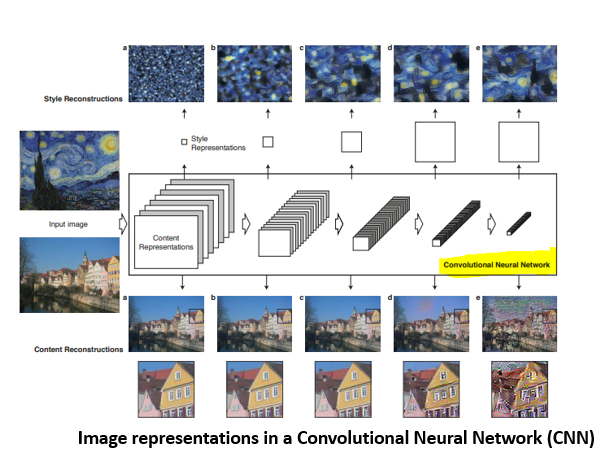
\includegraphics[width=0.5\textwidth]{assets/visualisasi-nst.png}
    \caption{\href{https://arxiv.org/pdf/1508.06576.pdf}{Visualisasi Proses NST}}
\end{figure*}

Pada algoritma \textit{Neural Style Transfer} (NST), \textit{Convolutional Neural Network} (CNN) berperan sebagai pemetaan dari piksel pada gambar ke fitur yang lebih memiliki makna. Setiap layer konvolusi dalam arsitektur VGG-19 menghasilkan himpunan \textit{feature map} yang dapat dipandang sebagai representasi berbeda dengan tingkat abstraksi yang meningkat seiring kedalaman layer. Secara umum, layer-layer awal cenderung menangkap pola lokal, seperti garis dan tekstur sederhana, sedangkan layer yang lebih dalam menangkap struktur global dan susunan objek dalam citra. 

Terdapat tiga buah citra utama yang penting, yaitu citra konten $I_c$, citra gaya $I_s$, dan citra hasil $I_g$. Citra konten $I_c$ adalah citra yang struktur semantiknya ingin dipertahankan, citra gaya $I_s$ adalah citra yang karakteristik artistiknya ingin ditransfer kepada citra $I_c$. Terakhir, citra hasil $I_g$ adalah citra yang menjadi variabel optimasi dan pada iterasi awal biasanya diinisialisasi sebagai citra konten $I_c$ atau citra noice acak.


Ketiga citra tersebut dimasukkan ke dalam jaringan VGG-19 yang bobotnya dibekukan, sehingga pada layer ke-$l$ masing-masing citra menghasilkan tensor fitur berdimensi berukuran $C_l \times H_l \times W_l$. Tensor-tensor ini kemudian di-\textit{flatten} dan dinyatakan sebagai matriks fitur
$$
F_c^l, F_s^l, F_g^l \in \mathbb{R}^{C_l \times (H_l \cdot W_l)}
$$
di mana tiap baris merepresentasikan satu kanal fitur dan setiap kolom merepresentasikan satu posisi spasial. Dengan demikian, pada layer ke-$l$, $F_c^l$ merupakan representasi fitur citra konten, $F_s^l$ merupakan representasi fitur citra gaya, dan $F_g^l$ merupakan representasi fitur citra hasil yang terus berubah seiring proses mengoptimasi $I_g$.

Pada representasi konten, informasi yang relevan adalah nilai aktivasi pada tiap posisi, sehingga jarak antara $F_c^l$ dan $F_g^l$ diukur langsung menggunakan norma Frobenius untuk mendefinisikan \textit{content loss}. Dengan demikian, konten dipandang sebagai pola aktivasi yang spesifik pada setiap lokasi dalam \textit{feature map}.

Dalam konteks pemisahan konten dan gaya, perbedaan karakteristik representasi ini dimanfaatkan untuk mendefinisikan dua jenis informasi yang ingin dipertahankan pada citra hasil $I_g$. Representasi konten biasanya diambil dari satu atau beberapa layer menengah yang dianggap cukup sensitif terhadap struktur global citra, tetapi tidak terlalu sensitif terhadap variasi tekstur lokal. Sebaliknya, representasi gaya diperoleh dari beberapa layer yang tersebar dari permukaan hingga kedalaman jaringan, sehingga dapat menangkap pola gaya pada berbagai posisi.


Berbeda dengan itu, representasi gaya diambil berdasarkan korelasi statistik antar fitur yang kemudian diringkas dalam bentuk Matriks Gram. Untuk setiap layer gaya ke-$l$, Matriks Gram $G_s^l$ dan $G_g^l$ dihitung dari $F_s^l$ dan $F_g^l$ sebagai
$$
G^l = F^l (F^l)^\top
$$
sehingga elemen $G_{ij}^l$ merepresentasikan inner product antara kanal ke-$i$ dan ke-$j$ yang mengukur tingkat keselarasan kedua fitur tersebut di seluruh posisi pada citra. Dengan cara ini, gaya tidak lagi bergantung pada posisi absolut di dalam citra, melainkan pada pola koaktivasi fitur yang bersifat lebih global. 

Pemilihan layer konten dan himpunan layer gaya tersebut tidak bersifat sembarang, melainkan dilihat dari pemahaman tentang bagaimana CNN menyandikan informai pada berbagai kedalaman jaringan. Layer yang terlalu dangkal jika digunakan sevagai representasi konten cenderung hanya mempertahankan detail lokal sehingga struktur semantik citra dapat terganggu, sedangkan layer gaya yang terlalu dalam berpotensi mengubah bentuk dalam porsi besar apabila Matriks Gram-nya dipaksakan untuk diikuti oleh citra hasil. Oleh karena itu, konfigurasi layer konten dan gaya dalam NST harus dipelajari secara mendalam sehingga kebutuhan mempertahankan struktur global citra konten dan karakteristik gaya dapat diseimbangkan dengan baik.


\subsection{Fungsi Loss pada Representasi Konten dan Gaya}
Setelah representasi konten dan gaya pada CNN didefinisikan melalui matriks fitur $F_c^l, F_s^l, F_g^l$ dan Matriks Gram, langkah berikutnya adalah menganalisis bagaimana fungsi loss membuat citra hasil $I_g$ mendekati citra konten dan citra gaya. Dalam konteks \textit{Neural Style Transfer} (NST), seluruh perilaku algoritma ditentukan oleh \textit{content loss}, \textit{style loss}, dan fungsi antar keduanya.

Representasi konten diambil dari matriks fitur $F_c^l$ dan $F_g^l$ pada layer ke-$i$, Secara intuitif, \textit{content loss} mengukur seberapa besar perbedaan antara citra hasil dan citra konten pada ruang fitur tersebut. Bentuk umum yang digunakan adalah
$$
\mathcal{L}_{content}^l = \frac{1}{2} \Vert F_g^l - F_c^l \Vert_F^2
$$

Jika $\mathcal{L}_{content}$ besar, berarti pola aktivasi $F_g^l$ berbeda jauh dari $F_c^l$, sehingga struktur objek dalam citra hasil mulai menyimpang dari citra konten. Sebaliknya, meminimalkan \textit{content loss} akan mendorong $F_g^l$ mendekati $F_c^l$, sehingga bentuk dan tata letak objek utama tetap terjaga. 

Berbeda dengan konten, gaya direpresentasikan melalui Matriks Gram yang menangkap korelasi antar fitur pada beberapa layer gaya yang dipilih. Untuk sebuah layer gaya ke-$l$, Matriks Gram $G_s^l$ dari citra gaya dan $G_g^l$ dari citra hasil didefinisikan dengan
$$
G_s^l = F_s^l (F_s^l)^\top, \hspace{1cm} G_g^l = F_g^l (F_g^l)^\top
$$
Lalu, \textit{style loss} pada layer tersebut kemudian diukur sebagai
$$
\mathcal{L}_{style}^l = \Vert G_g^l - G_s^l \Vert_F^2
$$
yang merepresentasikan seberapa jauh korelasi fitur citra hasil menyimpang dari korelasi fitur gaya. Nilai $\mathcal{L}_{\text{style}}^l$ yang kecil menunjukkan bahwa pola tekstur, warna, dan koaktivasi fitur pada $I_g$ mirip dengan $I_s$, terlepas dari posisi spasial gaya tersebut.

Dalam praktiknya, gaya tidak hanya diambil dari satu layer, tetapi dari himpunan layer $\mathcal{S}$ yang tersebar dai awal hingga akhir jaringan untuk menangkap gaya pada berbagai skala. \textit{Style loss} total biasanya dirumuskan sebagai
$$
\mathcal{L}_{style} = \sum_{l \in \mathcal{S}} w_l \mathcal{L}^l_{style}
$$

dengan $w_l$ adalah bobot kontribusi layer ke-$l$. Pemilihan dan pembobotan layer mempengaruhi seberapa halus atau kasarnya tekstur gaya yang muncul pada citra hasil.

Terakhir, untuk menghasilkan citra baru yang gayanya diambil dari $I_s$ dan kontennya dari $I_c$. Fungsi loss total biasanya ditulis dengan
$$
\mathcal{L}_{total} (I_g) = \alpha \mathcal{L}_{content}(I_g) + \beta \mathcal{L}_{style} (I_g)
$$

dengan $\alpha > 0$ dan $\beta > 0$ adalah hiperparameter yang mengatur keseimbangan antara preservasi konten dan intensitas gaya. Nilai $\alpha$ yang relatif besar akan menekankan kesesuaian konten, sehingga citra hasil cenderung mempertahankan struktur $I_c$ tetapi mungkin hanya mengadopsi gaya secara halus. Sebaliknya, nilai $\beta$ yang jauh lebih besar mendorong citra hasil untuk mengikuti Matriks Gram citra gaya secara agresif, sehingga tekstur dan warna gaya menjadi dominan tetapi struktur konten bisa mengalami distorsi.

\subsection{Optimasi Hasil Fungsi Loss terhadap Akurasi Citra Hasil Akhir}
Setelah \textit{content loss} dan \textit{style loss} dirumuskan, rekayasa citra hasil $I_g$ dilakukan melalui optimasi iteratif berbasis gradien terhadap piksel $I_g$. Ide utama dari menemukan \textit{content loss} dan \textit{style loss} minimum adalah dengan memperlakukan $I_g$ sebagai variabel bebas yang diubah sedikit demi sedikit sehingga $\mathcal{L}_{content}(I_g)$ dan $\mathcal{L}_{style}(I_g)$ sama-sama mengecil dan citra hasil menjadi semakin mirip dengan konten dan gaya yang diinginkan.

Optimasi menggunakan gradien ini digunakan dengan cara menghitung gradien total terhadap $I_g$ yang dihitung dengan menggunakan langkah-langkah berikut.
\begin{IEEEenumerate}
    \item Nyatakan gradien total sebagai penjumlahan berbobot gradien komponen konten dan gaya:
    $$
      \nabla_{I_g} \mathcal{L}_{\text{total}}
        = \alpha \, \nabla_{I_g} \mathcal{L}_{\text{content}}
        + \beta \, \nabla_{I_g} \mathcal{L}_{\text{style}}.
    $$
\item Hitung masing-masing gradien $\nabla_{I_g} \mathcal{L}_{\text{content}}$ dan $\nabla_{I_g} \mathcal{L}_{\text{style}}$ dengan menggunakan turunan parsial dan aturan rantai, yaitu dengan \textit{backtracking} gradien dari ruang fitur dan Matriks Gram kembali ke ruang piksel $I_g$ melalui jaringan CNN. ($\partial \frac{\mathcal{L}_{total}}{\partial I_g}$)
    \item Perbarui $I_g$ sedikit ke arah $-\nabla_{I_g} \mathcal{L}_{\text{total}}$ untuk menurunkan nilai loss. Secara umum, pembaruan ini dapat ditulis sebagai
    $$
        I_g^{(t+1)} = I_g^{(t)} - \eta \, \nabla_{I_g} \mathcal{L}_{\text{total}}(I_g^{(t)}),
    $$
    dengan $\eta$ menyatakan \emph{learning rate} atau langkah pembaruan yang diatur oleh algoritma optimasi (misalnya gradient descent, Adam, atau L-BFGS).
\end{IEEEenumerate}

\subsection{Peran Hiperparameter $\alpha$ dan $\beta$ dalam Fungsi Loss}

Hiperparameter $\alpha$ dan $\beta$ pada fungsi loss total
$$
\mathcal{L}_{total}(I_g) = \alpha \mathcal{L}_{content}(I_g) + \beta \mathcal{L}_{style}(I_g)
$$

berperan sebagai pengatur keseimbangan antara preservasi konten dna intensitas gaya pada citra hasil $I_g$. Nilai relatif antara $\alpha$ dan $\beta$ menentukan seberapa kuat gradien yang berasal dari \textit{content loss} dibandingkan gradien yang berasal dari \textit{style loss} dalam proses optimasi berbasis gradien. Dengan demikian, pemilihan $\alpha$ dan $\beta$ menjadi komponen penting dalam mendesain hasil akhir dari algoritma NST.

Secara intuitif, $\alpha$ yang lebih besar daripada $\beta$ membuat algoritma lebih condong ke arah citra konten $I_c$, sehingga struktur objek, posisi, dan bentuk pada $I_g$ cenderung lebih mirip dengan $I_c$. Pada konfigurasi ini, gaya dari $I_s$ umumnya hanya muncul sebagai modifikasi halus pada warna atau tekstur permukaan, tanpa mengubah secara signifikan geometri konten. Sebaliknya, jika $\beta$ dibuat jauh lebih besar daripada $\alpha$ membuat algoritma lebih condong ke arah citra gaya $I_s$, sehingga pola tekstur, palet warna, dan komponen gaya lain dari $I_g$ cenderung lebih mirip dengan $I_s$, meskipun terkadang dengan mengorbankan kejelasan struktur konten. 

Dalam berbagai implementasi NST, sering digunakan rasio $\beta \gg \alpha$, misalnya dengan menetapkan $\alpha = 1$ dan $\beta$ dalam orde $10^3$ atau lebih, untuk menghasilkan gaya yang cukup menonjol namun tetap mempertahankan konten secara global. Rasio ini biasanya tidak dipilih secara teoretis murni, melainkan melalui eksperimen dan "konvensi" dari berbagai literatur. Secara praktis, proses tuning dapat dilakukan dengan mengamati hasil visual: jika konten banyak hilang karena gaya, maka $\alpha$ dapat dinaikkan atau $\beta$ diturunkan; sebaliknya, jika gaya terasa terlalu lemah, $\beta$ dapat dinaikkan relatif terhadap $\alpha$.

\subsection{Proses Optimasi Iteratif terhadap Citra Hasil}

Proses optimasi pada algoritma \textit{Neural Style Transfer} berlangsung secara iteratif dengan memperbarui citra hasil $I_g$ agar \textit{content loss} dan \textit{style loss} secara bersamaan menurun dari waktu ke waktu. Pada iterasi awal, perbedaan antara representasi fitur citra hasil terhadap citra konten dan citra gaya masih besar, sehingga nilai $\mathcal{L}_{\text{total}}(I_g)$ relatif tinggi dan gradien yang dihasilkan juga cenderung memiliki magnitudo besar. Hal ini menyebabkan perubahan visual pada $I_g$ antar iterasi terlihat cukup drastis. Seiring bertambahnya iterasi, $I_g$ perlahan-lahan bergerak menuju konfigurasi yang lebih seimbang, di mana konten dan gaya semakin jelas namun tidak lagi berubah secara ekstrem di setiap iterasi.

Dari sudut pandang optimasi berbasis gradien, dinamika ini dapat dipahami melalui perubahan gradien $\nabla_{I_g} \mathcal{L}_{\text{total}}$ terhadap iterasi. Ketika $I_g$ masih jauh dari minimum lokal, komponen gradien yang berasal dari $\mathcal{L}_{\text{content}}$ dan $\mathcal{L}_{\text{style}}$ sama-sama besar sehingga langkah pembaruan $I_g^{(t+1)} = I_g^{(t)} - \eta \nabla_{I_g} \mathcal{L}_{\text{total}}(I_g^{(t)})$ menghasilkan pergeseran signifikan di ruang piksel. Namun, ketika $I_g$ mendekati titik kesetimbangan antara konten dan gaya, selisih $F_g^l - F_c^l$ dan $G_g^l - G_s^l$ secara bertahap mengecil, sehingga gradien yang dihitung melalui aturan rantai menjadi semakin kecil pula. Akibatnya, perubahan $I_g$ antar iterasi akhir menjadi halus, dan citra hasil tak banyak berubah secara visual meskipun masih ada penyesuaian kecil pada tekstur dan warna.

\subsection{Keterkaitan Komponen Aljabar Linier dengan Algoritma NST}

Algoritma \textit{Neural Style Transfer} pada dasarnya dapat dipandang sebagai rangkaian operasi aljabar linier yang diterapkan pada representasi citra dalam bentuk tensor. Setiap tahap utama, mulai dari representasi citra digital, ekstraksi fitur oleh CNN, pembentukan Matriks Gram, hingga perumusan fungsi \textit{loss} dan proses optimasi, selalu melibatkan konsep dasar, seperti ruang vektor, \textit{inner product}, norma, dan transformasi linier. Dengan demikian, kemampuan NST dan menggabungkan kembali konten dan gaya bukan hanya bergantung pada arsitektur \textit{neural network}, tetapi juga pada struktur matematis yang disediakan oleh aljabar linier. 

Representasi citra saebagai tensor $I \in \mathbb{R}^{H \times W \times C}$ memungkinkan setiap citra dipandang sebagai elemen dalam ruang vektor atau matriks berdimensi tinggi, di mana operasi dasar, seperti penjumlahan, perkalian skalar, dan transformasi linier masih dapat diterapkan. Proses ekstraksi fitur oleh CNN pada dasarnya adalah penerapan berulang dari transformasi linier. Hal ini dikarenakan konvolusi dalam CNN dapat dinyatakan sebagai perkalian matriks atau operator linier lainnya sesuai kebutuhan. Lalu, di akhir proses CNN hasil dari konvolusi diikuti oleh fungsi aktivasi nonlinier. Hasilnya adalah matriks fitur $F_c^l, F_s^l, F_g^l \in \mathbb{R}^{C_l \times (H_l W_l)}$ yang masing-masing merubah citra konten, gaya, dan hasil ke dalam basis fitur yang sama, sehingga perbandingan dan pengukuran jarak antar ketiganya dapat dilakukan secara alami dalam ruang vektor yang sama.

Matriks Gram muncul sebagai komponen kunci yang menjembatani konsep korelasi fitur dengan representasi gaya. Dengan membentuk $G^l = F^l (F^l)^\top$, algoritma NST memanfaatkan inner product antar baris $F^l$ untuk menangkap hubungan geometris antar kanal fitur, sehingga $G^l$ dapat ditafsirkan sebagai matriks korelasi yang bersifat simetris dan positive semi-definite. Sifat-sifat aljabar linier dari Matriks Gram, seperti kemampuan untuk didiagonalisasi secara orthogonal dan interpretasi nilai eigen sebagai komponen gaya yang dominan, memberikan landasan teoretis mengapa $G_s^l$ dan $G_g^l$ yang serupa akan menghasilkan tekstur dan pola gaya yang sejenis pada citra. Dengan kata lain, gaya artistik direduksi menjadi Matriks Gram sehingga dapat dimanipulasi menggunakan aljabar linier.

Perumusan fungsi loss dalam NST juga sangat bergantung pada konsep jarak dalam ruang vektor dan ruang matriks. Content loss didefinisikan sebagai jarak kuadrat (norma Frobenius) antara matriks fitur $F_c^l$ dan $F_g^l$, yang merupakan generalisasi dari jarak Euclidean antara dua vektor yang sebelumnya diperkenalkan dalam konteks fungsi loss dan MSE. Demikian pula, style loss mengukur jarak antara Matriks Gram $G_s^l$ dan $G_g^l$ dengan menggunakan norma Frobenius, sehingga secara eksplisit menghitung perbedaan gaya dan korelasi antar fitur yang diformulasikan sebagai selisih dua matriks dalam ruang $\mathbb{R}^{C_l \times C_l}$. Penggunaan norma Frobenius sebagai ukuran kesalahan menjamin bahwa fungsi loss bersifat non-negatif dan terdiferensialkan, sehingga cocok digunakan dalam skema optimasi berbasis gradien.

Terakhir, proses optimasi iteratif terhadap citra hasil $I_g$ memanfaatkan turunan parsial dan aturan rantai untuk menghitung gradien $\nabla_{I_g} \mathcal{L}_{\text{total}}$, yang secara konseptual merupakan elemen lain dari struktur aljabar linier, meskipun dalam proses pembelajaran IF2123 Aljabar Linier dan Geometri tidak diajarkan. Melalui backpropagation, gradien yang semula dihitung di ruang fitur ($F_g^l$) dan ruang Matriks Gram ($G_g^l$) ditarik kembali ke ruang piksel $I_g$ dengan menerapkan komposisi transformasi linier yang mendeskripsikan layer-layer CNN. 

Setiap iterasi
$$
I_g^{(t+1)} = I_g^{(t)} - \eta \,\nabla_{I_g} \mathcal{L}_{\text{total}}(I_g^{(t)})
$$
dapat dipandang sebagai perpindahan vektor dalam ruang citra yang mengarah ke titik minimum lokal (titik di mana nilai fungsi \textit{loss} paling kecil), di mana titik tersebut merepresentasikan titik keseimbangan dari dua hiperparameter $\alpha$ dan $\beta$ antara kesesuaian konten dan kesesuaian gaya. Dengan demikian, algoritma NST bukan hanya prosedur komputasional menggunakan CNN, tetapi merupakan contoh penerapan tingkat tinggi dari konsep-konsep aljabar linier. Mulai dari representasi citra menggunakan tensor, pembentukan Matriks Gram, perhitungan fungsi loss dan gradien, semuanya merupakan konsep-konsep aljabar linier yang digabungkan sehingga bersama-sama dapat melakukan sintesis gaya sebuah citra dan menggabungkannya dengan citra konten. 

\section{Kesimpulan}

Algoritma \textit{Neural Style Network} (NST) yang nampak kompleks dan menggunakan istilah yang rumit ternyata hanya merupakan penerapan konsep-konsep Aljabar Linier tingkat tinggi. Dalam sintesis citra artistik, aljabar linier yang digunakan mulai dari Matriks Gram dan \textit{Convolutional Neural Network} (NST) sebenarnya hanya hasil abstraksi dari konsep-konsep aljabar linier dasar. Representasi citra digital dapat dipandang sebagai sebuah matriks dan/atau tensor berdimensi tinggi, telah dibahas bahwa setiap citra dapat dipandang sebagai elemen dalam ruang vektor sehingga operasi untuk aljabar vektor dapat diterapkan. Lalu, setelah dipetakan/direpresentasikan menggunakan vektor dan tensor, CNN dapat digunakan untuk memetakan ruang piksel menjadi ruang fitur, di mana setiap layer menghasilkan \textit{feature map} yang merepresentasikan citra pada layer abstraksi yang berbeda.

Dalam konteks NST, citra utama yang dipertimbangkan adalah citra konten $I_c$, citra gaya $I_s$, dan citra hasil $I_g$ yang digunakan sebagai variabel optimasi. Ketiganya dimasukkan ke dalam jaringan CNN VGG-19 sehingga pada leyer-layer tertentu diperoleh matriks fitur $F_c^l, F_s^l, F_g^l$ yang membaca konten dan gaya dalam basis yang sama. Di mana jaringan CNN ini sebenarnya hanyalah transformasi linier (yang dapat direpresentasikan oleh sebuah matriks) yang dilakukan dalam beberapa layer.

Representasi konten didefinisikan sebagai pola aktivasi pada \textit{feature map}, sehingga \textit{content loss} dapat dihitung dengan menghitung jarak kuadrat (norma Frobenius) antara $F_c^l$ dan $F_g^l$ untuk memastikan citra hasil mendekati citra konten. Sedangkan, representasi gaya diperoleh melalui Matriks Gram $G_s^l$ dan $G_g^l$ yang dibentuk dari \textit{inner product} antar fitur pada beberapa layer gaya. Matriks Gram dapat menangkan korelasi statistik antar fitur dan bersifat simetris, sehingga dapat dipandang sebagai matriks korelasi berisikan tekstur, pola, dan palet warna dari sebuah citra gaya, tanpa bergantung pada posisi aktual dari detail gaya tersebut. Sama, seperti pada \textit{content loss}, \textit{style loss} dapat dihitung menggunakan jarak kuadrat antara Matriks Gram dari citra hasil dan Matriks Gram dari citra gaya.

Sementara itu, representasi gaya diperoleh melalui Matriks Gram $G_s^l$ dan $G_g^l$ yang dibentuk dari inner product antar kanal fitur pada beberapa layer gaya. Matriks Gram ini menangkap korelasi statistik antar fitur dan bersifat simetris serta positive semi-definite, sehingga dapat dipandang sebagai matriks korelasi yang menyandikan tekstur, pola, dan palet warna citra gaya tanpa bergantung pada posisi spasial detail tersebut. Style loss kemudian dirumuskan sebagai jarak antara Gram matrix citra hasil dan citra gaya, sehingga meminimalkan style loss akan memaksa korelasi fitur $I_g$ mengikuti pola korelasi $I_s$.

Terakhir, kedua komponen loss tersebut digabungkan dalam persamaan \textit{loss total}, 
$$
L_{\text{total}}(I_g) = \alpha L_{\text{content}}(I_g) + \beta L_{\text{style}}(I_g)
$$

dengan hiperparameter $\alpha$ dan $\beta$ yang mengatur trade-off intensitas gaya dan konten. Proses optimasi dilakukan secara iteratif dengan menghitung gradien $\nabla_{I_g} L_{\text{total}}$ terhadap piksel $I_g$ melalui aturan rantai dan backpropagation, kemudian memperbarui $I_g$ sedikit demi sedikit dengan skema optimasi berbasis gradien hingga diperoleh citra hasil yang secara visual menggabungkan konten $I_c$ dan gaya $I_s$.

Dari sudut pandang Aljabar Linier, keseluruhan algoritma NST menunjukkan bagaimana representasi citra sebagai tensor, operasi matriks (termasuk transpos, perkalian, dan pembentukan Matriks Gram), konsep inner product dan norma, serta perhitungan gradien berperan langsung dalam memformulasikan dan menyelesaikan masalah pemisahan dan penggabungan konten-gaya pada citra digital. Dengan demikian, NST dapat dipandang sebagai contoh nyata bagaimana teori ruang vektor dan transformasi linier diaplikasikan untuk menghasilkan sintesis citra artistik yang kompleks namun tetap didasarkan pada struktur matematis yang jelas dan terukur.


\begin{thebibliography}{99}

\bibitem{gatys2015}
L.~A. Gatys, A.~S. Ecker, and M.~Bethge, ``A neural algorithm of artistic style,'' in \emph{Proc. IEEE Conf. Comput. Vis. Pattern Recognit. (CVPR)}, 2016, pp. 2414--2423. [Online]. Available: \url{https://arxiv.org/abs/1508.06576}. Accessed: Dec. 10, 2025.

\bibitem{if2123_site}
R.~Munir, ``IF2123 Aljabar Linier dan Geometri,'' Program Studi Teknik Informatika, Institut Teknologi Bandung, 2025. [Online]. Available: \url{https://informatika.stei.itb.ac.id/~rinaldi.munir/AljabarGeometri/}. Accessed: Dec. 10, 2025.

\bibitem{gfg_dip}
GeeksforGeeks, ``Digital image processing basics,'' Feb. 13, 2023. [Online]. Available: \url{https://www.geeksforgeeks.org/computer-graphics/digital-image-processing-basics/}. Accessed: Dec. 10, 2025.

\bibitem{vgg19}
K.~Simonyan and A.~Zisserman, ``Very deep convolutional networks for large-scale image recognition,'' in \emph{Proc. Int. Conf. Learn. Represent. (ICLR)}, 2015. [Online]. Available: \url{https://arxiv.org/abs/1409.1556}. Accessed: Dec. 11, 2025.

\bibitem{datacamp}
S.~Paul, ``Implementing neural style transfer using TensorFlow 2.0,'' DataCamp, 2019. [Online]. Available: \url{https://www.datacamp.com/tutorial/implementing-neural-style-transfer-using-tensorflow}. Accessed: Dec. 12, 2025.

\bibitem{aldo}
A.~Ferlatti, ``Neural style transfer (NST) — theory and implementation,'' Medium, 2021. [Online]. Available: \url{https://medium.com/@ferlatti.aldo/neural-style-transfer-nst-theory-and-implementation-c26728cf969d}. Accessed: Dec. 12, 2025.

\bibitem{ml4a}
G.~G. Author, ``Style transfer,'' in \emph{Machine Learning for Artists}, 2016. [Online]. Available: \url{https://ml4a.github.io/ml4a/style_transfer/}. Accessed: Dec. 13, 2025.

\bibitem{yt_gram}
Why Gram Matrix in Style Transfer || Quick Explained, YouTube, Dec. 2020. [Online]. Available: \url{https://www.youtube.com/watch?v=Elxnzxk-AUk}. Accessed: Dec. 13, 2025.

\bibitem{gfg_cnn}
GeeksforGeeks, ``Introduction to convolution neural network,'' Jul. 11, 2025. [Online]. Available: \url{https://www.geeksforgeeks.org/machine-learning/introduction-convolution-neural-network/}. Accessed: Dec. 24, 2025.

\bibitem{wandb}
Weights \& Biases, ``Exploring neural style transfer with Weights \& Biases,'' Sept. 2023. [Online]. Available: \href{https://wandb.ai/wandb_fc/articles/reports/Exploring-Neural-Style-Transfer-with-Weights-Biases--Vmlldzo1NDM1MjA2}{Exploring neural style transfer with Weights \& Biases}. Accessed: Dec. 24, 2025.

\bibitem{amit_gram}
A.~Agrawal, ``How does Gram matrix encode the style of an image?,'' 2017. [Online]. Available: \url{http://amit-agrawal.com/NN-1-20171201.html}. Accessed: Dec. 24, 2025.

\bibitem{harley_cnnviz}
A.~W. Harley, ``An interactive node-link visualization of convolutional neural networks,'' in \emph{Advances in Visual Computing (ISVC 2015)}, 2015, pp. 867--877.

\end{thebibliography}


\section*{Ucapan Terima Kasih dan Kata Hati}
Penulis mengucapkan syukur kepada Tuhan Yang Maha Esa atas rahmat dan karunia-Nya sehingga makalah ini dapat diselesaikan dengan baik. Ucapan terima kasih yang sebesar-besarnya penulis sampaikan kepada Bapak Dr. Ir. Rinaldi, M.T. selaku dosen pengampu mata kuliah IF2123 Aljabar Linier dan Geometri yang telah memberikan penjelasan dan materi yang sangat membantu dalam memahami konsep dasar Aljabar Linier dan Geometri dan keterkaitannya di bidang Informatika. Penulis juga menyampaikan terima kasih kepada jajaran Asisten IRK STEI ITB yang sudah menyusun segala tugas besar dan soal kuis yang penuh pembelajaran. Tidak lupa, penulis menghargai teman-teman penulis yang dalam proses pembelajaran, stres, dan \textit{crash out} yang dialami selama mata kuliah ini, mereka selalu senantiasa berada di samping penulis dengan penuh cemoohan dan kasih sayang.

Makalah ini membahas tentang penerapan konsep-konsep tingkat tinggi Aljabar Linier baik yang diajarkan di dalam ruang kelas IF2123 Aljabar Linier dan Geometri, maupun tidak. Adapun penyesalan penulis karena memilih topik yang cukup kompleks, berhubung dengan waktu yang dimiliki penulis tidak sebanyak teman-teman lain, karena sedang melaksanakan rangkaian ibadah Umroh. Hampir setengah makalah ini ditulis di luar tanah air, sesuai mimpi penulis yang ingin menulis baris-baris kode untuk bekerja di bidang Informatika di luar negara Indonesia, tetapi nyatanya dengan waktu yang terbatas, semuanya tidak seindah apa yang dimimpikan. Akan tetapi, penulis bahagia bisa menyelesaikan makalah ini tepat pada waktunya dan akhirnya menyelesaikan mata kuliah IF2123 Aljabar Linier dan Geometri. Semoga pembelajaran yang didapat di mata kuliah ini bisa menjadi pelajaran berharga baik secara akademik, maupun nonakademik.

Keberjalanan mata kuliah ini sungguh memberikan pembelajaran yang membuka mata hati, saya belajar bahwa usaha belajar lebih dari 12 jam, tidak selalu memberikan nilai maksimal, malah kadang hanya memberikan nilai sesuai fungsi berikut.
$$
F(\mathcal{W}_h) = \eta \times \mathcal{W}_h
$$
dengan $\eta$ adalah koefisien waktu belajar (biasanya 4 atau 5) dan $\mathcal{W}_h$ adalah waktu yang dihabiskan untuk belajar dalam satuan jam. Sehingga menghasilkan $F$ yang menjadi nilai ujian/kuis yang didapatkan. Misal dengan $\eta = 4$ dan waktu belajar $\mathcal{W}_h = 12$ biasanya penulis mendapatkan nilai $F(\mathcal{W}_h) = 48$. Sekiranya ini hanyalah estimasi dan nilai penulis alhamdulillah tidak sejelek itu (MUNGKIN).

\pagebreak
\section*{Pernyataan}
Dengan ini saya menyatakan bahwa makalah yang saya tulis
ini adalah tulisan saya sendiri, bukan saduran, atau terjemahan
dari makalah orang lain, dan bukan plagiasi. Pada halaman selanjutnya juga saya lampirkan surat pernyataan penggunaan AI yang saya gunakan dalam mengerjakan tugas ini.

\vspace*{1em}
\raggedleft
Kapadokia, 24 Desember 2025

\begin{figure}[H]
    \raggedleft
    
\includegraphics[width=0.13\textwidth]{assets/ttd endra.jpg}
    \hspace{1cm}
\end{figure}

\raggedleft
Narendra Dharma Wistara M. \\
13524044

\onecolumn 
\section*{\textbf{Surat Pernyataan Penggunaan AI}}
\justifying
\noindent Dengan ini, saya:
\begin{tabbing}
    Program Studi \hspace{1.5cm} \= : \hspace{0.5cm} \= \kill
    \indent Nama                    \> : \> Narendra Dharma Wistara M. / 13524044 \\
    \indent Fakultas/Sekolah        \> : \> Sekolah Teknik Elektro dan Informatika - Komputasi\\
    \indent Program Studi           \> : \> Teknik Informatika \\
    \indent Kode Mata Kuliah        \> : \> IF2123 \\
    \indent Nama Mata Kuliah        \> : \> Aljabar Linier dan Geometri \\
    \indent Judul Tugas/Proposal    \> : \> Analisis Penggunaan Gram Matrix dan CNN dalam Algoritma Neural Style Transfer untuk \\
    \> \> Sintesis Citra Artistik
\end{tabbing}

\noindent Menyatakan bahwa saya menggunakan AI dalam pengerjaan maupun penyusunan luaran tugas pada mata kuliah yang tertulis di atas. Alat AI/kecerdasan buatan yang digunakan adalah: 

\begin{table}[htbp]
\begin{center}
    \normalsize
\begin{tabular}{|p{0.62\linewidth}|p{0.15\linewidth}|p{0.15\linewidth}|}
\hline

\parbox[c][4em][c]{\linewidth}{\centering \textbf{Lingkup Pekerjaan}} & 
\parbox[c][4em][c]{\linewidth}{\centering \textbf{Digunakan?}} & 
\parbox[c][4em][c]{\linewidth}{\centering \textbf{Tingkat Penggunaan}} \\
\hline

\textbf{Pemeriksaan Ejaan:} menggunakan tools seperti Grammarly, Paperpal, Deepl, Quillbot, Grammarbot, LanguageTool, ProWritingAid, ChatGPT, Google Gemini, atau sejenisnya &
Ya & 
Rendah \\
\hline

\textbf{Pembuatan Teks:} menggunakan tools seperti ChatGPT, Gemini, Paperpal, Copilot, GrammarlyGo, WordAI, WriteSonic, Jasper, Jenni AI, atau sejenisnya. &
Ya & 
Rendah \\
\hline

\textbf{Bantuan Diskusi dalam Penyusunan Konten:} menggunakan tools seperti ChatGPT, Gemini, Copilot, Perplexity, Jenni AI, Zoom-Companion, atau sejenisnya. &
Tidak &
- \\
\hline

\textbf{Pembuatan Gambar, Video, dan/atau Grafik:} menggunakan tools seperti Craiyon, DALL-E, Midjourney, Stable Diffusion, Microsoft Designer, Gemini, Canva AI, atau sejenisnya. &
Tidak &
- \\
\hline

\textbf{Pencarian Referensi: } menggunakan tools, seperti Perplexity, Gemini, atau sejenisnya. &
Ya &
Sedang \\
\hline

\textbf{Translasi Referensi Berbahasa Asing: } menggunakan tools, seperti Perplexity, Gemini, atau sejenisnya. &
Ya &
Rendah \\
\hline

\end{tabular}
\end{center}
\end{table}

\noindent Saya juga menyatakan bahwa setiap penggunaan AI/kecerdasan buatan yang dilakukan pada mata kuliah tersebut telah dinyatakan di dalam surat ini.

\begin{flushright}
    Kapadokia, 24 Desember 2025 \\
    Penulis, 
    \begin{figure}[H]
    \raggedleft
    
\includegraphics[width=0.12\textwidth]{assets/ttd endra.jpg}
    \hspace{1cm}
\end{figure}
    Narendra Dharma Wistara M. \\
    13524044
\end{flushright}

\vfill 


\end{document}
